\begin{frame}
\frametitle{Training quiz and certificate}
\begin{itemize}
\item You have been given a quiz to test your knowledge
      on the topics covered by the course.
      That's not too late to take it if you haven't done it yet!
\item At the end of the course, we will submit this quiz
      to you again. That time, you will see the correct answers.
\item It allows Bootlin to assess your progress thanks to the course.
      That's also a kind of challenge, to look for clues throughout
      the lectures and labs / demos, as all the answers are in the course!
\item Another reason is that we only give training certificates
      to people who achieve at least a 50\% score in the final quiz
      {\bf and} who attended all the sessions.
\end{itemize}
\end{frame}

\begin{frame}

\frametitle{Participate!}
During the lectures...
\begin{itemize}
\item Don't hesitate to ask questions. Other people in the audience may have
similar questions too.
\item Don't hesitate to share your experience too, for example to compare Linux
with other operating systems you know.
\item Your point of view is most valuable, because it can be similar to your
colleagues' and different from the trainer's.
\item In on-line sessions
   \begin{itemize}
   \item Please keep your camera on too if you have one.
   \item Also make sure your name is properly filled.
   \item If Jitsi Meet is used, you can also use the "Raise your hand"
         button when you wish to ask a question but don't want to
	 interrupt.
   \end{itemize}
\item All this helps the trainer to engage with participants, see when
something needs clarifying and make the session more interactive, enjoyable
and useful for everyone.
\end{itemize}
\end{frame}

\begin{frame}
\frametitle{Collaborate!}
\begin{columns}
\column{0.8\textwidth}
  As in the Free Software and Open Source community,
  collaboration between participants is valuable in this training session:
  \begin{itemize}
    \item Use the dedicated Matrix channel for this session
	  to add questions.
    \item If your session offers practical labs, you can also
          report issues, share screenshots and command output there.
    \item Don't hesitate to share your own answers and to help others
          especially when the trainer is unavailable.
    \item The Matrix channel is also a good place to ask questions
	  outside of training hours, and after the course is over.
    \end{itemize}
\column{0.2\textwidth}
  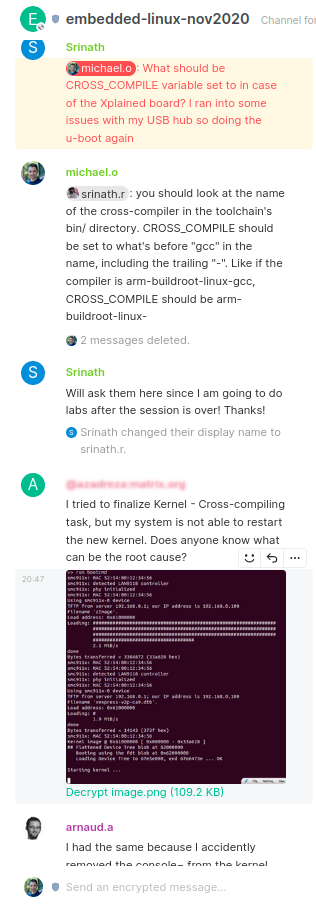
\includegraphics[height=0.8\textheight]{slides/course-information/matrix-screenshot.png}
\end{columns}
\end{frame}
